% Options for packages loaded elsewhere
\PassOptionsToPackage{unicode}{hyperref}
\PassOptionsToPackage{hyphens}{url}
%
\documentclass[
]{article}
\usepackage{lmodern}
\usepackage{amssymb,amsmath}
\usepackage{ifxetex,ifluatex}
\ifnum 0\ifxetex 1\fi\ifluatex 1\fi=0 % if pdftex
  \usepackage[T1]{fontenc}
  \usepackage[utf8]{inputenc}
  \usepackage{textcomp} % provide euro and other symbols
\else % if luatex or xetex
  \usepackage{unicode-math}
  \defaultfontfeatures{Scale=MatchLowercase}
  \defaultfontfeatures[\rmfamily]{Ligatures=TeX,Scale=1}
\fi
% Use upquote if available, for straight quotes in verbatim environments
\IfFileExists{upquote.sty}{\usepackage{upquote}}{}
\IfFileExists{microtype.sty}{% use microtype if available
  \usepackage[]{microtype}
  \UseMicrotypeSet[protrusion]{basicmath} % disable protrusion for tt fonts
}{}
\makeatletter
\@ifundefined{KOMAClassName}{% if non-KOMA class
  \IfFileExists{parskip.sty}{%
    \usepackage{parskip}
  }{% else
    \setlength{\parindent}{0pt}
    \setlength{\parskip}{6pt plus 2pt minus 1pt}}
}{% if KOMA class
  \KOMAoptions{parskip=half}}
\makeatother
\usepackage{xcolor}
\IfFileExists{xurl.sty}{\usepackage{xurl}}{} % add URL line breaks if available
\IfFileExists{bookmark.sty}{\usepackage{bookmark}}{\usepackage{hyperref}}
\hypersetup{
  pdftitle={Qiqi Xie's CV},
  pdfauthor={Qiqi Xie},
  hidelinks,
  pdfcreator={LaTeX via pandoc}}
\urlstyle{same} % disable monospaced font for URLs
\usepackage[margin=1in]{geometry}
\usepackage{graphicx}
\makeatletter
\def\maxwidth{\ifdim\Gin@nat@width>\linewidth\linewidth\else\Gin@nat@width\fi}
\def\maxheight{\ifdim\Gin@nat@height>\textheight\textheight\else\Gin@nat@height\fi}
\makeatother
% Scale images if necessary, so that they will not overflow the page
% margins by default, and it is still possible to overwrite the defaults
% using explicit options in \includegraphics[width, height, ...]{}
\setkeys{Gin}{width=\maxwidth,height=\maxheight,keepaspectratio}
% Set default figure placement to htbp
\makeatletter
\def\fps@figure{htbp}
\makeatother
\setlength{\emergencystretch}{3em} % prevent overfull lines
\providecommand{\tightlist}{%
  \setlength{\itemsep}{0pt}\setlength{\parskip}{0pt}}
\setcounter{secnumdepth}{-\maxdimen} % remove section numbering

\title{Qiqi Xie's CV}
\author{Qiqi Xie}
\date{2020-06-04}

\begin{document}
\maketitle

\hypertarget{aside}{%
\section{Aside}\label{aside}}

\begin{figure}
\centering
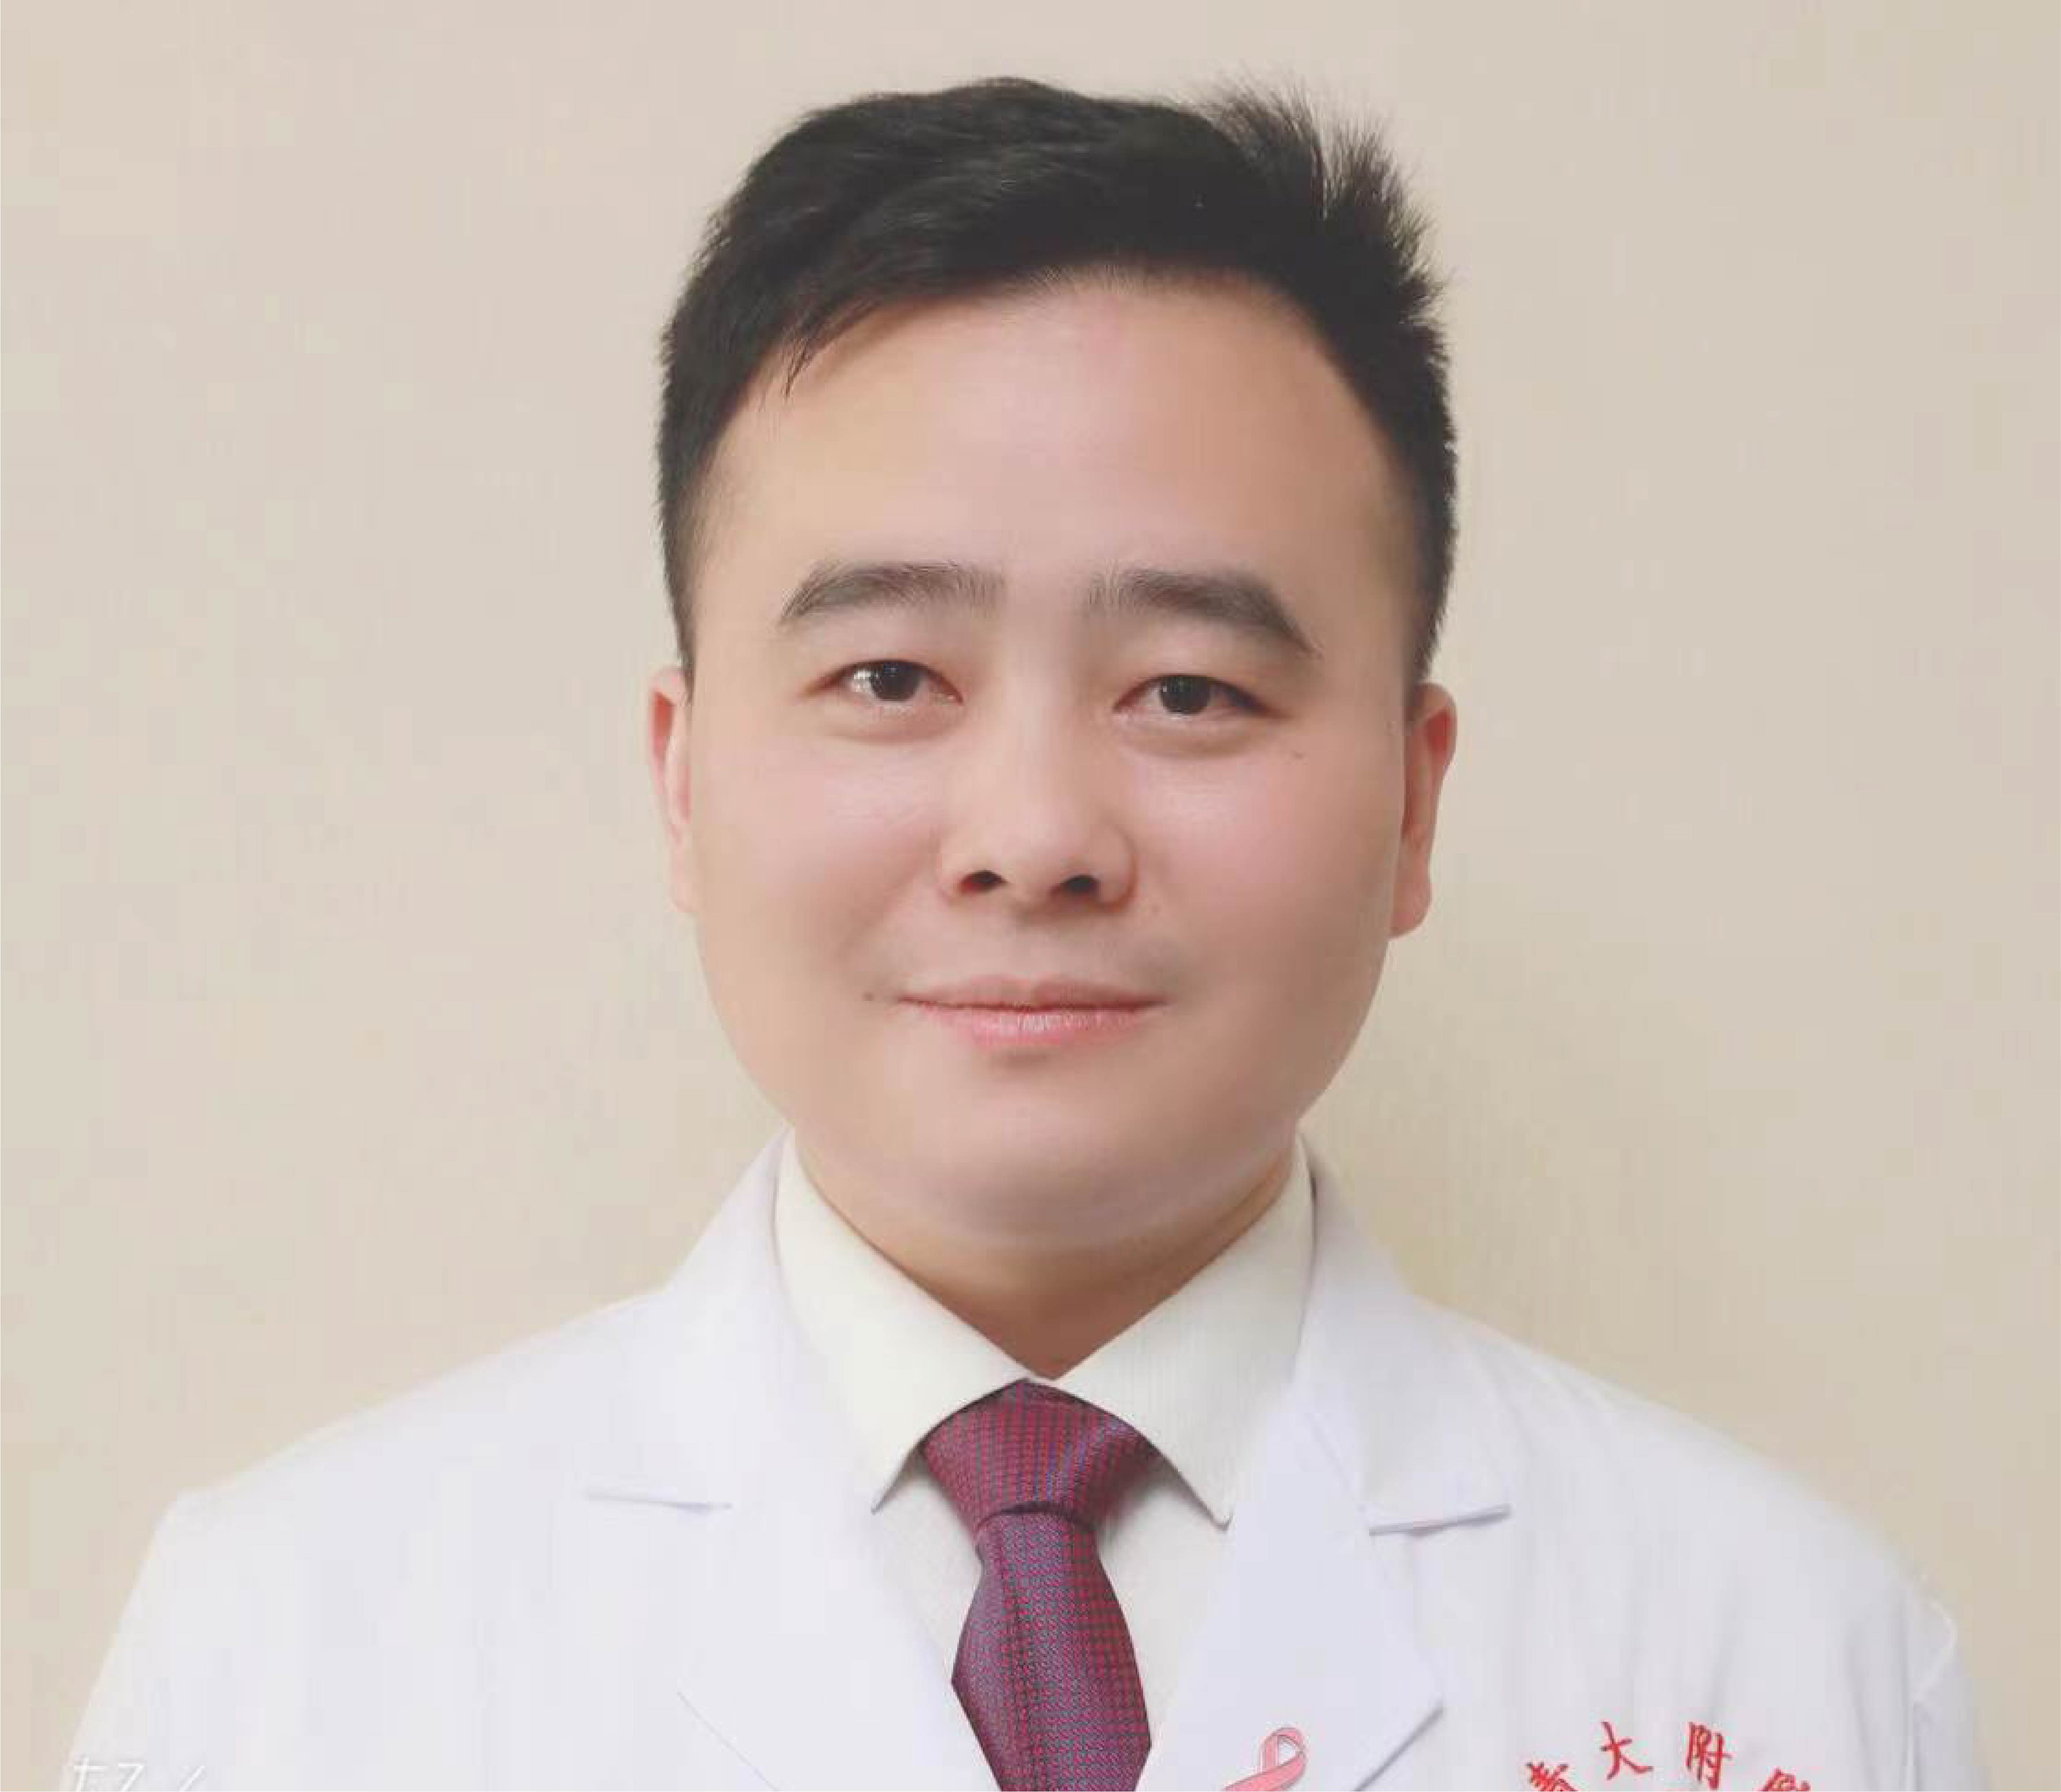
\includegraphics[width=1\textwidth,height=\textheight]{xqq.jpg}
\caption{logo}
\end{figure}

\hypertarget{contact}{%
\subsection{Contact}\label{contact}}

\begin{itemize}
\tightlist
\item
  \href{mailto:jieqq16@lzu.edu.cn}{\nolinkurl{jieqq16@lzu.edu.cn}}
\item
  QiqiXie
\item
  \url{https://github.com/Qiqi-Xie}
\item
  \url{https://orcid.org/0000-0003-4099-5287}
\item
  lcy505264
\item
  (86) 15719612948
\end{itemize}

\hypertarget{main}{%
\section{Main}\label{main}}

\hypertarget{title}{%
\subsection{Qiqi Xie}\label{title}}

Bioinformatics Scientist. Data scientist. Biologist. Master of Medicine.
Fluent in Bioinformatics, NGS analysis, and machine learning.

I am broadly interested in bone tumor, osteoporosis, osteoarthritis, and
neuropathic pain. Currently searching for a PhD position that allows me
to do some meaningful research.

\hypertarget{education}{%
\subsection{Education}\label{education}}

\hypertarget{master-of-orthopedics}{%
\subsubsection{Master of Orthopedics}\label{master-of-orthopedics}}

Lanzhou University

Gansu, CN

2019 - 2016

\begin{itemize}
\tightlist
\item
  Mechanism of TRPM2-GSK3\textless U+00A6\textgreater{} Signaling
  Pathway in Diabetic Osteoporosis
\end{itemize}

\hypertarget{diploma-of-clinical-medicine}{%
\subsubsection{Diploma of Clinical
Medicine}\label{diploma-of-clinical-medicine}}

Nanchang University

Jiangxi, CN

2015 - 2010

\hypertarget{certificate}{%
\subsection{Certificate}\label{certificate}}

\hypertarget{outstanding-graduates}{%
\subsubsection{Outstanding Graduates}\label{outstanding-graduates}}

N/A

Lanzhou University

2018

\hypertarget{national-scholarships}{%
\subsubsection{National Scholarships}\label{national-scholarships}}

N/A

Lanzhou University

\hypertarget{the-first-prize-scholarship}{%
\subsubsection{The First-Prize
Scholarship}\label{the-first-prize-scholarship}}

N/A

Lanzhou University

\hypertarget{the-third-prize-scholarship}{%
\subsubsection{The Third-Prize
Scholarship}\label{the-third-prize-scholarship}}

N/A

Lanzhou University

2016

\hypertarget{the-third-prize-scholarship-1}{%
\subsubsection{The Third-Prize
Scholarship}\label{the-third-prize-scholarship-1}}

N/A

Nanchang University

2014

\hypertarget{the-second-prize-scholarship}{%
\subsubsection{The Second-Prize
Scholarship}\label{the-second-prize-scholarship}}

N/A

Nanchang University

2012

\hypertarget{national-college-english-competition-encouragement-award}{%
\subsubsection{National College English Competition Encouragement
Award}\label{national-college-english-competition-encouragement-award}}

N/A

Nanchang University

2011

\hypertarget{grants}{%
\subsection{Grants}\label{grants}}

\hypertarget{pain-mechanism-and-treatment-of-spinal-diseases}{%
\subsubsection{Pain mechanism and treatment of spinal
diseases}\label{pain-mechanism-and-treatment-of-spinal-diseases}}

participation

N/A

2019

\hypertarget{the-mechanism-of-exosome-micrornas-in-osteoporosis}{%
\subsubsection{The mechanism of exosome microRNAs in
osteoporosis}\label{the-mechanism-of-exosome-micrornas-in-osteoporosis}}

participation

N/A

2019 - 2018

\hypertarget{mechanism-of-trpm2-gsk3u00a6-signaling-pathway-in-diabetic-osteoporosis}{%
\subsubsection{Mechanism of TRPM2-GSK3\textless U+00A6\textgreater{}
Signaling Pathway in Diabetic
Osteoporosis}\label{mechanism-of-trpm2-gsk3u00a6-signaling-pathway-in-diabetic-osteoporosis}}

participation

N/A

2018 - 2017

\hypertarget{endogenous-cannabinoids-regulate-astrocyte-mediated-pain-the-mapk-glu-gln-shuttle-pathway}{%
\subsubsection{Endogenous cannabinoids regulate astrocyte-mediated pain:
the MAPK-Glu-Gln shuttle
pathway}\label{endogenous-cannabinoids-regulate-astrocyte-mediated-pain-the-mapk-glu-gln-shuttle-pathway}}

participation

N/A

2017 - 2016

\hypertarget{publications}{%
\subsection{Publications}\label{publications}}

\hypertarget{decreased-expression-of-nusap1-predicts-poor-overall-survival-in-cervical-cancer}{%
\subsubsection{\texorpdfstring{\href{https://www.jcancer.org/v11p2852.htm}{Decreased
expression of NUSAP1 predicts poor overall survival in cervical
cancer}}{Decreased expression of NUSAP1 predicts poor overall survival in cervical cancer}}\label{decreased-expression-of-nusap1-predicts-poor-overall-survival-in-cervical-cancer}}

\emph{\textbf{Journal of Cancer}}

N/A

2020

\begin{itemize}
\tightlist
\item
  \textbf{Qiqi Xie}, Wen Ou-yang, Mingwei Zhang, Huimei Wang, Qiuyuan
  Yue\textsuperscript{*}
\end{itemize}

\hypertarget{identification-of-a-novel-autophagy-related-gene-signature-for-predicting-metastasis-and-survival-in-patients-with-osteosarcoma}{%
\subsubsection{\texorpdfstring{\href{https://www.researchsquare.com/article/rs-19384/v1}{Identification
of a novel autophagy-related gene signature for predicting metastasis
and survival in patients with
osteosarcoma}}{Identification of a novel autophagy-related gene signature for predicting metastasis and survival in patients with osteosarcoma}}\label{identification-of-a-novel-autophagy-related-gene-signature-for-predicting-metastasis-and-survival-in-patients-with-osteosarcoma}}

\emph{\textbf{Research Square}}

N/A

\begin{itemize}
\tightlist
\item
  Guangzhi Zhang, Yajun Deng, Zuolong Wu, Enhui Ren, Wenhua Yuan,
  \emph{Qiqi Xie}\textsuperscript{*}
\end{itemize}

\hypertarget{protein-kinase-a-is-involved-in-neuropathic-pain-by-activating-the-p38mapk-pathway-to-mediate-spinal-cord-cell-apoptosis}{%
\subsubsection{\texorpdfstring{\href{https://doi.org/10.1155/2020/6420425}{Protein
Kinase A Is Involved in Neuropathic Pain by Activating the p38MAPK
Pathway to Mediate Spinal Cord Cell
Apoptosis}}{Protein Kinase A Is Involved in Neuropathic Pain by Activating the p38MAPK Pathway to Mediate Spinal Cord Cell Apoptosis}}\label{protein-kinase-a-is-involved-in-neuropathic-pain-by-activating-the-p38mapk-pathway-to-mediate-spinal-cord-cell-apoptosis}}

\emph{\textbf{Mediators of Inflammation}}

N/A

\begin{itemize}
\tightlist
\item
  Yajun Deng, Liang Yang, \textbf{Qiqi Xie}, Fengbiao Yang, Guoqiang Li,
  Guangzhi Zhang, Shaoping Li, Zuolong Wu, Jing Wang, Xuewen
  Kang\textsuperscript{*}
\end{itemize}

\hypertarget{mcm2-and-nusap1-are-potential-biomarkers-for-the-diagnosis-and-prognosis-of-pancreatic-cancer}{%
\subsubsection{\texorpdfstring{\href{https://doi.org/10.1155/2020/8604340}{MCM2
and NUSAP1 Are Potential Biomarkers for the Diagnosis and Prognosis of
Pancreatic
Cancer}}{MCM2 and NUSAP1 Are Potential Biomarkers for the Diagnosis and Prognosis of Pancreatic Cancer}}\label{mcm2-and-nusap1-are-potential-biomarkers-for-the-diagnosis-and-prognosis-of-pancreatic-cancer}}

\textbf{\emph{BioMed Research International}}

N/A

\begin{itemize}
\tightlist
\item
  Yajun Deng, Hanyun Ma, Jinyong Hao\textsuperscript{*}, \textbf{Qiqi
  Xie}\textsuperscript{*}, Ruochen Zhao\textsuperscript{*}
\end{itemize}

\hypertarget{grb10-and-e2f3-as-diagnostic-markers-of-osteoarthritis-and-their-correlation-with-immune-infiltration}{%
\subsubsection{\texorpdfstring{\href{https://doi.org/10.3390/diagnostics10030171}{GRB10
and E2F3 as Diagnostic Markers of Osteoarthritis and Their Correlation
with Immune
Infiltration}}{GRB10 and E2F3 as Diagnostic Markers of Osteoarthritis and Their Correlation with Immune Infiltration}}\label{grb10-and-e2f3-as-diagnostic-markers-of-osteoarthritis-and-their-correlation-with-immune-infiltration}}

\textbf{\emph{Diagnostics}}

N/A

\begin{itemize}
\tightlist
\item
  Yajun Deng, Enhui Ren, Wenhua Yuan , Guangzhi Zhang, Zuolong Wu,
  \textbf{Qiqi Xie}\textsuperscript{*}
\end{itemize}

\hypertarget{identification-of-diagnostic-markers-for-major-depressive-disorder-by-cross-validation-of-data-from-whole-blood-samples}{%
\subsubsection{\texorpdfstring{\href{https://peerj.com/articles/7171/}{Identification
of diagnostic markers for major depressive disorder by cross-validation
of data from whole blood
samples}}{Identification of diagnostic markers for major depressive disorder by cross-validation of data from whole blood samples}}\label{identification-of-diagnostic-markers-for-major-depressive-disorder-by-cross-validation-of-data-from-whole-blood-samples}}

\textbf{\emph{PeerJ}}

N/A

2019

\begin{itemize}
\tightlist
\item
  Huimei Wang\_, Mingwei Zhang\_, \textbf{Qiqi Xie}, Jin Yu, Yan Qi\_,
  Qiuyuan Yue\textsuperscript{*}
\end{itemize}

\hypertarget{anterior-versus-posterior-decompression-for-the-treatment-of-thoracolumbar-fractures-with-spinal-cord-injurya-meta-analysis}{%
\subsubsection{\texorpdfstring{\href{https://doi.org/10.3969/j.issn.1003-0034.2019.03.015}{Anterior
versus posterior decompression for the treatment of thoracolumbar
fractures with spinal cord injury:a
Meta-analysis}}{Anterior versus posterior decompression for the treatment of thoracolumbar fractures with spinal cord injury:a Meta-analysis}}\label{anterior-versus-posterior-decompression-for-the-treatment-of-thoracolumbar-fractures-with-spinal-cord-injurya-meta-analysis}}

\textbf{\emph{China journal of orthopaedics and traumatology}}

N/A

\begin{itemize}
\tightlist
\item
  Enhui Ren, Yajun Deng, \textbf{Qiqi Xie}, Liang Yang, Guangzhi Zhang,
  Shaoping Li, Zuolong Wu, Jing Wang, Xuewen Kang\textsuperscript{*}
\end{itemize}

\hypertarget{identification-of-potential-diagnostic-and-therapeutic-target-genes-for-lung-squamous-cell-carcinoma}{%
\subsubsection{\texorpdfstring{\href{https://doi.org/10.3892/ol.2019.10300}{Identification
of potential diagnostic and therapeutic target genes for lung squamous
cell
carcinoma}}{Identification of potential diagnostic and therapeutic target genes for lung squamous cell carcinoma}}\label{identification-of-potential-diagnostic-and-therapeutic-target-genes-for-lung-squamous-cell-carcinoma}}

\textbf{\emph{Oncology Letters}}

N/A

\begin{itemize}
\tightlist
\item
  Nana Zhang, Hong Wang, \textbf{Qiqi Xie}, Hua Cao, Fanqi Wu, Dan Bei
  Di Wu, Yixin Wan\textsuperscript{*}
\end{itemize}

\hypertarget{integrative-analyses-of-genes-associated-with-idiopathic-pulmonary-fibrosis}{%
\subsubsection{\texorpdfstring{\href{https://doi.org/10.1002/jcb.28153}{Integrative
analyses of genes associated with idiopathic pulmonary
fibrosis}}{Integrative analyses of genes associated with idiopathic pulmonary fibrosis}}\label{integrative-analyses-of-genes-associated-with-idiopathic-pulmonary-fibrosis}}

\textbf{\emph{Journal of Cellular Biochemistry}}

N/A

\begin{itemize}
\tightlist
\item
  Huimei Wang, \textbf{Qiqi Xie}, Wen Ou\_Yang, Mingwei
  Zhang\textsuperscript{*}
\end{itemize}

\hypertarget{slow-skeletal-muscle-troponin-t-titin-and-myosin-light-chain-3-are-candidate-prognostic-biomarkers-for-ewings-sarcoma}{%
\subsubsection{\texorpdfstring{\href{https://doi.org/10.3892/ol.2019.11044}{Slow
skeletal muscle troponin T, titin and myosin light chain 3 are candidate
prognostic biomarkers for Ewing's
sarcoma}}{Slow skeletal muscle troponin T, titin and myosin light chain 3 are candidate prognostic biomarkers for Ewing's sarcoma}}\label{slow-skeletal-muscle-troponin-t-titin-and-myosin-light-chain-3-are-candidate-prognostic-biomarkers-for-ewings-sarcoma}}

\textbf{\emph{Oncology Letters}}

N/A

\begin{itemize}
\tightlist
\item
  Yajun Deng, \textbf{Qiqi Xie}, Guangzhi Zhang, Shaoping Li, Zuolong
  Wu, Zhanjun Ma, Xuegang He, Yicheng Gao, Yonggang Wang, Xuewen Kang,
  Jing Wang\textsuperscript{*}
\end{itemize}

\hypertarget{arachidonyl-glycerol-modulates-astrocytic-glutamine-synthetase-via-p38-and-erk12-pathways}{%
\subsubsection{\texorpdfstring{\href{https://doi.org/10.1186/s12974-018-1254-x}{2-arachidonyl
glycerol modulates astrocytic glutamine synthetase via p38 and ERK1/2
pathways}}{2-arachidonyl glycerol modulates astrocytic glutamine synthetase via p38 and ERK1/2 pathways}}\label{arachidonyl-glycerol-modulates-astrocytic-glutamine-synthetase-via-p38-and-erk12-pathways}}

\textbf{\emph{Journal of Neuroinflammation}}

N/A

\begin{itemize}
\tightlist
\item
  Shenghong Wang, Hua Zhang, Bin Geng, \textbf{Qiqi Xie}, Wenzhou Li,
  Yajun Deng, Weidong Shi, Yunyan Pan, Xuewen Kang, Jing
  Wang\textsuperscript{*}
\end{itemize}

\hypertarget{high-affinity-glutamate-transporters-and-chronic-pain}{%
\subsubsection{\texorpdfstring{\href{https://doi.org/10.11817/j.issn.1672-7347.2017.09.016}{High-affinity
glutamate transporters and chronic
pain}}{High-affinity glutamate transporters and chronic pain}}\label{high-affinity-glutamate-transporters-and-chronic-pain}}

\textbf{\emph{Journal of Central South University (Medical Sciences)}}

N/A

\begin{itemize}
\tightlist
\item
  Zhang H, Wang S, \textbf{Xie Q}, Li W, Shi W, Ma J, Wang
  J\textsuperscript{*}
\item
  article in chinese
\end{itemize}

\hypertarget{bioinformatics-analysis-of-gene-chip-data-related-to-early-pathological-pain-induced-by-sni-rat-model}{%
\subsubsection{Bioinformatics analysis of gene chip data related to
early pathological pain induced by SNI rat
model}\label{bioinformatics-analysis-of-gene-chip-data-related-to-early-pathological-pain-induced-by-sni-rat-model}}

\textbf{\emph{Life Science Research}}

N/A

2018

\begin{itemize}
\tightlist
\item
  \textbf{Xie Q}, Li W, Shi W, Deng Y, Ren E, Ma J, Kang X, Wang
  J\textsuperscript{*}
\item
  article in chinese
\end{itemize}

\hypertarget{advances-in-application-of-gemstone-energy-spectrum-ct-in-skeletal-system}{%
\subsubsection{Advances in application of gemstone energy spectrum CT in
skeletal
system}\label{advances-in-application-of-gemstone-energy-spectrum-ct-in-skeletal-system}}

\textbf{\emph{Life science Research}}

N/A

\begin{itemize}
\tightlist
\item
  \textbf{Xie Q}, Li W, Shi W, Deng Y, Ren E, Ma J, Kang X, Wang
  J\textsuperscript{*}
\item
  article in chinese
\end{itemize}

\hypertarget{bioinformatics-analysis-of-osteoarthritis-expression-profile-microarray-integration}{%
\subsubsection{Bioinformatics analysis of osteoarthritis expression
profile microarray
integration}\label{bioinformatics-analysis-of-osteoarthritis-expression-profile-microarray-integration}}

\textbf{\emph{Hua Zhong Ke Ji Da Xue Xue Bao Yi Xue Ban}}

N/A

\begin{itemize}
\tightlist
\item
  \textbf{Xie Q}, Li W, Shi W, Deng Y, Ren E, Ma J, Kang X, Wang
  J\textsuperscript{*}
\item
  article in chinese
\end{itemize}

\hypertarget{effects-of-diabetes-on-bone-biomechanics-in-ovariectomized-rats}{%
\subsubsection{Effects of diabetes on bone biomechanics in
ovariectomized
rats}\label{effects-of-diabetes-on-bone-biomechanics-in-ovariectomized-rats}}

\textbf{\emph{Chinese Journal of Medical Physics}}

N/A

\begin{itemize}
\tightlist
\item
  \textbf{Xie Q}, Li W, Shi W, Deng Y, Ren E, Ma J, Pan Y, Kang X, Wang
  J\textsuperscript{*}
\item
  article in chinese
\end{itemize}

\hypertarget{selection-of-sites-for-detecting-bone-mineral-density-in-diabetic-osteoporosis-rats-by-dxa}{%
\subsubsection{Selection of sites for detecting bone mineral density in
diabetic osteoporosis rats by
DXA}\label{selection-of-sites-for-detecting-bone-mineral-density-in-diabetic-osteoporosis-rats-by-dxa}}

\textbf{\emph{Chinese Journal of Medical Physics}}

N/A

\begin{itemize}
\tightlist
\item
  Li W, \textbf{Xie Q}, Ren E, Deng Y, Pan Y, Ma J, Kang X, Wang
  J\textsuperscript{*}
\item
  article in chinese
\end{itemize}

\hypertarget{visual-analysis-of-related-literature-on-quantitative-computed-tomography-in-diagnosis-of-osteoporosis}{%
\subsubsection{Visual analysis of related literature on quantitative
computed tomography in diagnosis of
osteoporosis}\label{visual-analysis-of-related-literature-on-quantitative-computed-tomography-in-diagnosis-of-osteoporosis}}

\textbf{\emph{Chinese Journal of Medical Physics}}

N/A

\begin{itemize}
\tightlist
\item
  Deng Y, \textbf{Xie Q}, Li W, Shi W, Ma J, Pan Y, Kang X, Wang
  J\textsuperscript{*}
\item
  article in chinese
\end{itemize}

\hypertarget{the-expression-and-clinical-significance-of-formyl-peptide-receptor-1-in-glioma-were-analyzed-based-on-bioinformatics}{%
\subsubsection{The expression and clinical significance of formyl
peptide receptor 1 in glioma were analyzed based on
bioinformatics}\label{the-expression-and-clinical-significance-of-formyl-peptide-receptor-1-in-glioma-were-analyzed-based-on-bioinformatics}}

\textbf{\emph{Cancer, aberration, mutation}}

N/A

\begin{itemize}
\tightlist
\item
  Dong Q, \textbf{Xie Q}, Hu J, Wang M, Yuan G, Pan Y\textsuperscript{*}
\item
  article in chinese
\end{itemize}

\hypertarget{the-correlation-between-quantitative-parameters-of-edct-and-bone-biomechanics}{%
\subsubsection{The correlation between quantitative parameters of EDCT
and bone
biomechanics}\label{the-correlation-between-quantitative-parameters-of-edct-and-bone-biomechanics}}

\textbf{\emph{Chinese Journal of Medical Physics}}

N/A

\begin{itemize}
\tightlist
\item
  Dong Q, \textbf{Xie Q}, Zhao R, Huang X, Li W, Zhang Y, Pan
  Y\textsuperscript{*}
\item
  article in chinese
\end{itemize}

\hypertarget{preliminary-study-on-the-evaluation-of-biomechanics-by-edct}{%
\subsubsection{Preliminary study on the evaluation of biomechanics by
EDCT}\label{preliminary-study-on-the-evaluation-of-biomechanics-by-edct}}

\textbf{\emph{Chinese Journal of Medical Physics}}

N/A

\begin{itemize}
\tightlist
\item
  Huang X, \textbf{Xie Q}, Deng Y, Zhao R, Dong Q, Zhou
  J\textsuperscript{*}
\item
  article in chinese
\end{itemize}

\hypertarget{progress-in-the-study-of-skeletal-endocrine-function}{%
\subsubsection{Progress in the study of skeletal endocrine
function}\label{progress-in-the-study-of-skeletal-endocrine-function}}

\textbf{\emph{Life science Research}}

N/A

\begin{itemize}
\tightlist
\item
  Li W, \textbf{Xie Q}, Shi W, Deng Y, Ma Y, Xie J, Kang X, Wang
  J\textsuperscript{*}
\item
  article in chinese
\end{itemize}

\hypertarget{conference-proceedings}{%
\subsection{Conference proceedings}\label{conference-proceedings}}

\hypertarget{the-3th-academic-conference-of-chinese-medical-association-on-osteoporosis-and-bone-mineral-salt}{%
\subsubsection{\texorpdfstring{The 3\textsuperscript{th} Academic
Conference of Chinese Medical Association on Osteoporosis and Bone
Mineral
Salt}{The 3th Academic Conference of Chinese Medical Association on Osteoporosis and Bone Mineral Salt}}\label{the-3th-academic-conference-of-chinese-medical-association-on-osteoporosis-and-bone-mineral-salt}}

N/A

Shanxi, CN

2018

\hypertarget{the-9th-international-symposium-on-osteoporosis-and-bone-mineral-salt-diseases}{%
\subsubsection{\texorpdfstring{The 9\textsuperscript{th} International
Symposium on Osteoporosis and Bone Mineral Salt
Diseases}{The 9th International Symposium on Osteoporosis and Bone Mineral Salt Diseases}}\label{the-9th-international-symposium-on-osteoporosis-and-bone-mineral-salt-diseases}}

N/A

Suzhou, CN

\hypertarget{the-13th-annual-congress-of-chinese-orthopaedic-association}{%
\subsubsection{\texorpdfstring{The 13\textsuperscript{th} Annual
Congress of Chinese Orthopaedic
Association}{The 13th Annual Congress of Chinese Orthopaedic Association}}\label{the-13th-annual-congress-of-chinese-orthopaedic-association}}

N/A

Xiamen, CN

\hypertarget{professional-skills}{%
\section{Professional skills}\label{professional-skills}}

\hypertarget{experimental}{%
\subsection{Experimental}\label{experimental}}

\begin{itemize}
\tightlist
\item
  Open-field test, Water Maze Test, Forced Swimming Test, Von Frey Hair
  test, Cold Hot Plate Test. Stereotactic injection,
  Immunohistochemistry, Immunofluorescence, Western blot, RT-PCR, RNAi,
  Exosome purification and identification.
\item
  micro-drop PCR system, automatic protein expression quantitative
  system, high-content live cell imaging quantitative analysis system,
  cell metabolic analyzers, etc.
\end{itemize}

\hypertarget{software}{%
\subsection{Software}\label{software}}

\begin{itemize}
\tightlist
\item
  I have advanced experience in using Microsoft Office, Illustrator,
  Photoshop, GraphPad Prism, SPSS, ImageJ, Image-Pro Plus, Cytoscape,
  Funrich.
\end{itemize}

\hypertarget{statistics}{%
\subsection{Statistics}\label{statistics}}

\begin{itemize}
\tightlist
\item
  I have moderate experience in using R for statistical modeling and
  data visualization.
\end{itemize}

\hypertarget{machine-learning}{%
\subsection{Machine learning}\label{machine-learning}}

\begin{itemize}
\tightlist
\item
  I know how to do machine learning (including deep learning) and have
  applied some technologies to my projects
\end{itemize}

\hypertarget{data-analysis}{%
\subsection{Data analysis}\label{data-analysis}}

\begin{itemize}
\tightlist
\item
  I have advanced experience in using R and Shell for data
  preprocessing, data cleaning and data interpretation.
\end{itemize}

\hypertarget{disclaimer}{%
\subsection{Disclaimer}\label{disclaimer}}

Last updated on 2020-06-04.

\end{document}
